\documentclass[12pt,a4paper]{report}
\usepackage[utf8]{inputenc}
\usepackage{amsmath}
\usepackage{amsfonts}
\usepackage{amssymb}
\usepackage{graphicx}
\usepackage{caption}
\usepackage{fancyhdr}
\usepackage{titlesec}
\usepackage[top=2in, bottom=0.4in, left=0.6in, right=0.6in]{geometry}
\usepackage{pdfpages}
\usepackage{tabularx}
\usepackage{sidecap}
\usepackage{subcaption}
\usepackage{float}
\usepackage{multirow}


\usepackage[french]{babel}


%Setting header parameters
\addtolength{\voffset}{-72pt}

\pagestyle{fancyplain}
\setlength{\headheight}{50pt}
\lhead{}
\chead{}
\rhead{}

\renewcommand{\headrule}{
	\begin{minipage}{\textwidth}
		\textsl{\footnotesize Rapport de projet informatique} \hfill \textbf{\nouppercase{\leftmark}} \\
		\vspace{-10pt}
		\hrule 
		\vspace{5pt}
		\textsl{\footnotesize Stratification adaptative vs randomized QMC} \hfill 
	\end{minipage}
	\vspace{10pt}
}


\sidecaptionvpos{figure}{c}

\newcommand{\partdiff}[2]{\frac{\partial #1}{\partial #2}}

\renewcommand{\chaptermark}[1]{\markboth{\thechapter.\ #1}{}}
\titleformat{\chapter}[hang]{\bf\huge}{\thechapter}{2pc}{} 
\titlespacing*{\chapter}{0pt}{-30pt}{25pt}

\setlength{\parindent}{0pt}



\newcommand{\function}[1]{\texttt{#1}}
\newcommand{\N}{\mathbb{N}}
\newcommand{\esp}[1]{\mathbb{E}\left[ #1 \right]}
\newcommand{\iid}{i.i.d.}

\def \directory {/home/jonathan/Programmation/C++/Projet_C++_S2/Images}

\author{Omar El-Euch, Jonathan Visbecq \\ Stratification adaptative vs randomized QMC}
\title{\centering Master Probabilités et Finance: \\ \textbf{Rapport de projet informatique}}
\begin{document}

\maketitle

\tableofcontents

\chapter{Présentation du sujet}

\section{Sujet}
Le sujet choisi est le suivant:
\begin{center}
\bf
	2.21 Stratification adaptative vs randomized QMC
\end{center}


Comparer les performances des méthodes de stratification exposées dans \cite{EJ08} et de QMC randomisées exposées dans \cite{Tu04} sur les exemples présentés dans \cite{EJ08}.


\section{Présentation mathématique des modèles}

\subsection{Quasi-Monte Carlo randomisé}

\subsection{Stratification adaptative}

\chapter{Tests numériques du code C++}

\section{Quasi-Monte Carlo randomisé}

\subsection{Comparaison des vitesses de convergence}


\begin{figure}[H]
\centering
	\begin{subfigure}[scale=1]{0.45\textwidth}
			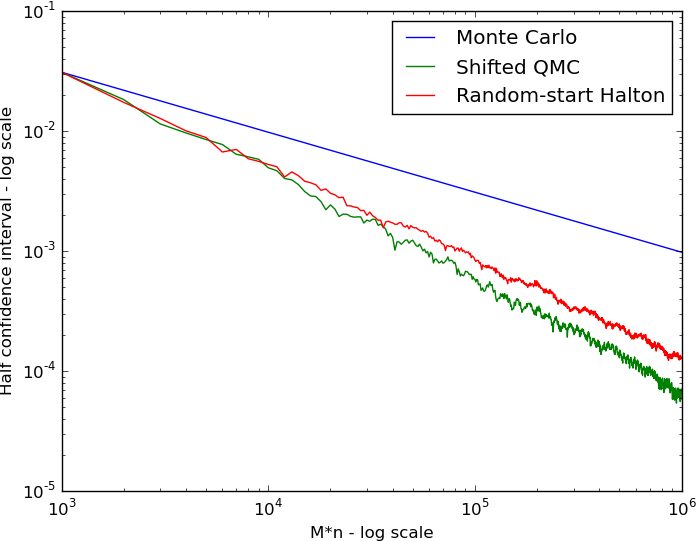
\includegraphics[scale=0.47]{\directory/compare_ciAndTime_MCvsRQMC__CI.png}
			\subcaption{Demi-interval de confiance en fonction du nombre de points générés (échelle 'log-log')}
	\end{subfigure}
	\hfill
	\begin{subfigure}[scale=1]{0.45\textwidth}
		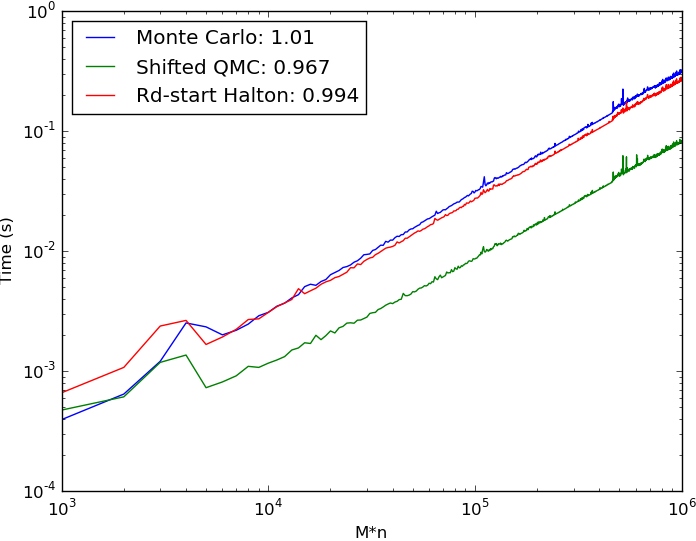
\includegraphics[scale=0.47]{\directory/compare_ciAndTime_MCvsRQMC__time.png}
		\subcaption{Temps (s) de calcul nécessaire en fonction du nombre de points générés (échelle 'log-log')}
	\end{subfigure}
	
\caption{\small Comparaison des temps et vitesses de convergence des méthodes de Monte Carlo randomisées et de Monte Carlo standard pour le calcul de l'intégrale de $f(x_{1},x_{2})=1_{x_{1}<x_{2}}$. M (nombre de pseudo-nombres aléatoires) est fixé à 1000 tandis que N (nombres de quasi-nombres aléatoires) varie de 1 à 1000. Les valeurs indiquées sont les coefficients des pentes (vitesses de convergences).}
\label{fig:rqmc_vitesse_convergence}
\end{figure}

\subsection{Étude du terme de Berry-Essen pour l'intervalle de confiance}
\begin{figure}[H]
\centering
	\begin{subfigure}[scale=1]{0.45\textwidth}
			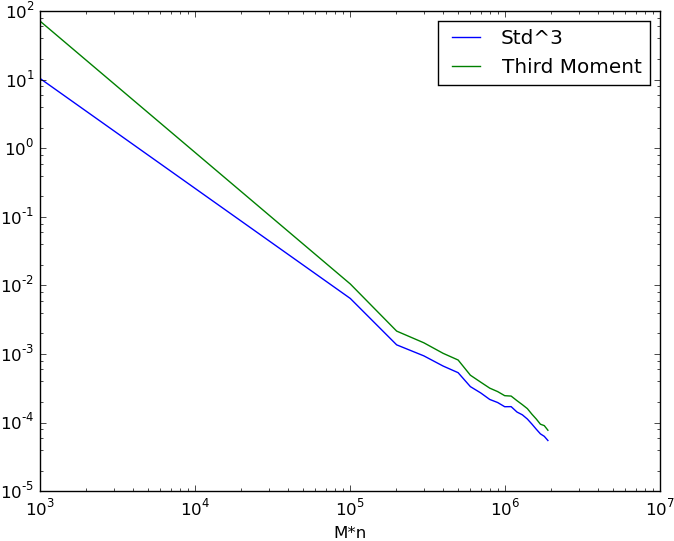
\includegraphics[scale=0.47]{\directory/compare_moments_func1_sqmc.png}
			\subcaption{$\prod_{i=1}^{10} \frac{\pi}{2} \sin(\pi x_{i})$} 
	\end{subfigure}
	\hfill
	\begin{subfigure}[scale=1]{0.45\textwidth}
			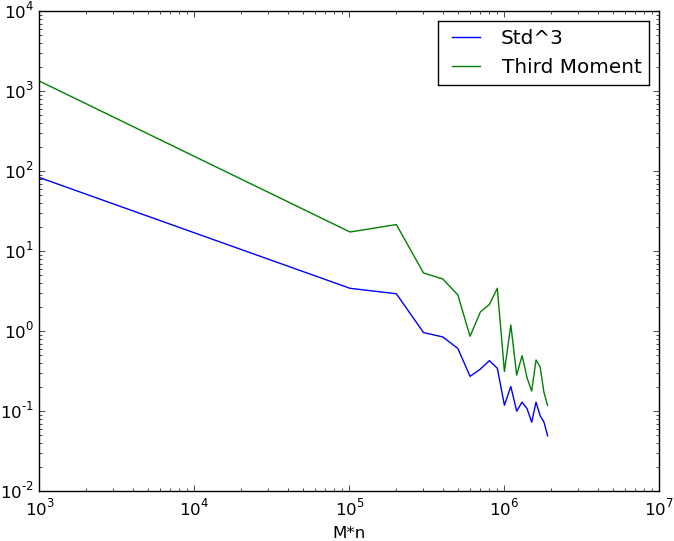
\includegraphics[scale=0.47]{\directory/compare_moments_func2_sqmc.png}
			\subcaption{$\prod_{i=1}^{10} 12(x_{i}-0.5)$} 
	\end{subfigure}
	\vspace{30pt}
	\begin{subfigure}[scale=1]{0.45\textwidth}
			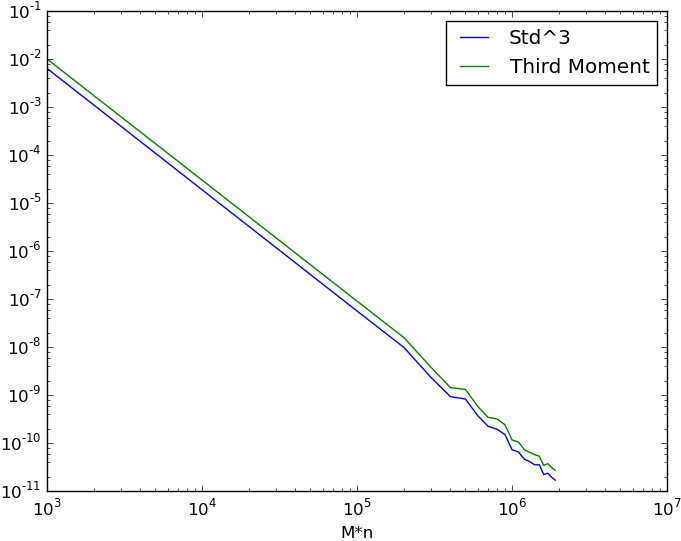
\includegraphics[scale=0.47]{\directory/compare_moments_func3_sqmc.png}
			\subcaption{$\frac{1}{5} \sum_{i=1}^{10} x_{i}$} 
	\end{subfigure}
	\hfill
	\begin{subfigure}[scale=1]{0.45\textwidth}
			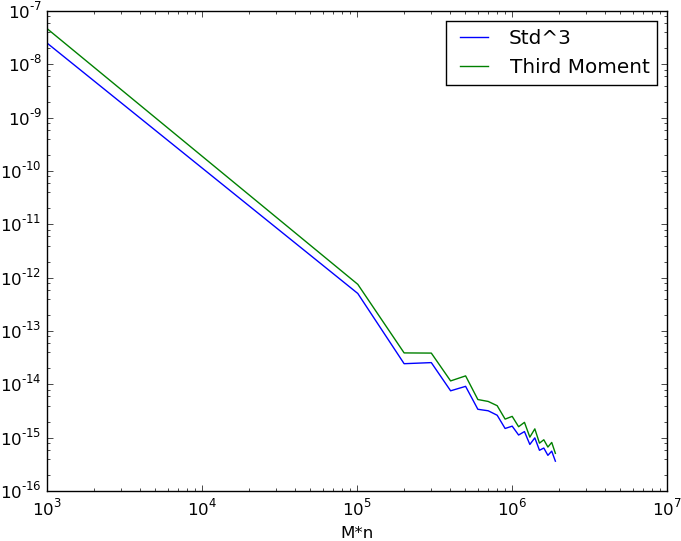
\includegraphics[scale=0.47]{\directory/compare_moments_func4_sqmc.png}
			\subcaption{$\prod_{i=1}^{10} \frac{e^{-|x_{i} - 0.5|}}{2-2e^{0.5}}$} 
	\end{subfigure}
	\vspace{30pt}
	\begin{subfigure}[scale=1]{0.45\textwidth}
			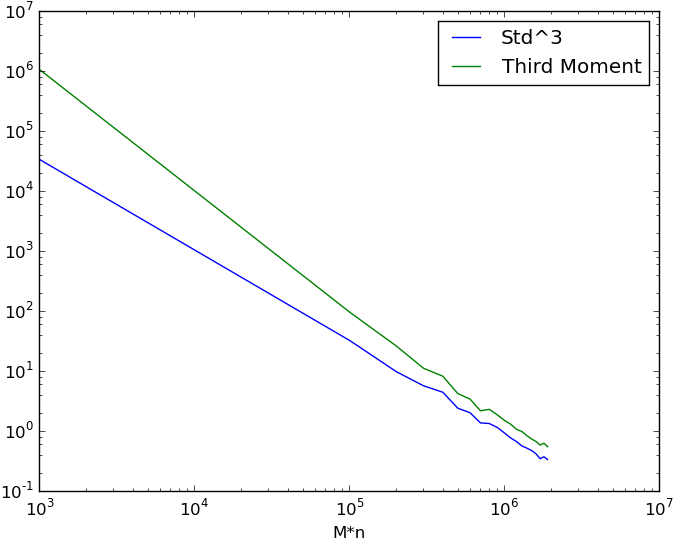
\includegraphics[scale=0.47]{\directory/compare_moments_func5_sqmc.png}
			\subcaption{$\prod_{i=1}^{10} 21_{\{x_{i}>0.5\}}$} 
	\end{subfigure}

	
\caption{\small Comparaison des vitesses de convergence de $\sigma^{3}_{N}$ et de $\beta_{N}$. Comme pour les simulations présentées dans \cite{Tu04}, la vitesse de convergence est sensiblement la même pour toutes les fonctions étudiées.}
\label{fig:rqmc_moments}
\end{figure}


\section{Stratification adaptative}

\subsection{Convergence vers la proportion optimale}

\begin{figure}[H]
\centering
	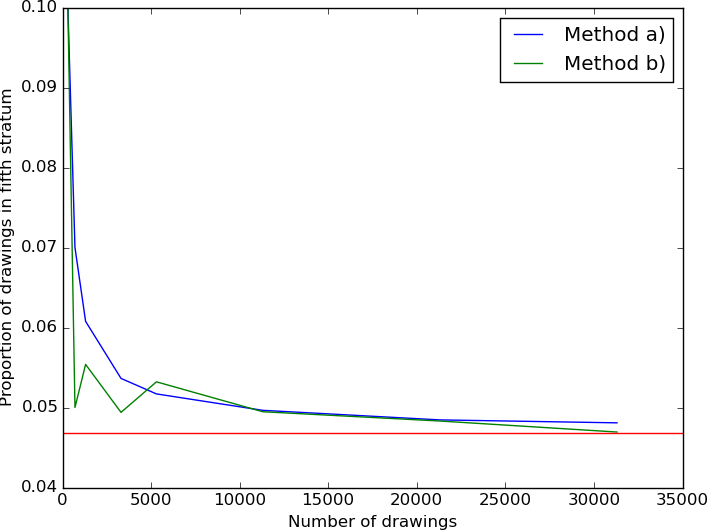
\includegraphics[scale=0.47]{\directory/stratification_reproduce_convergence.png}
	
\caption{\small Convergence de $\frac{N^{k}_{5}}{N^{k}}$ vers la valeur optimale $q_{5}^{*} = 0.04685$ (droite rouge) en fonction de $N^{k}$, pour $k \in [|1,8|]$ et $N^{k}$ prenant les valeurs 300, 700, 1300, 3300, 5300, 11300, 21300, 31300. Les deux méthodes de calcul possible pour la stratification adaptative sont envisagées.}
\label{fig:strat_convergence_proportion}
\end{figure}

\subsection{Comparaison de l'intervalle de confiance estimé à la simulation Monte Carlo}

\begin{figure}[H]
\centering
	\begin{subfigure}[scale=1]{0.45\textwidth}
			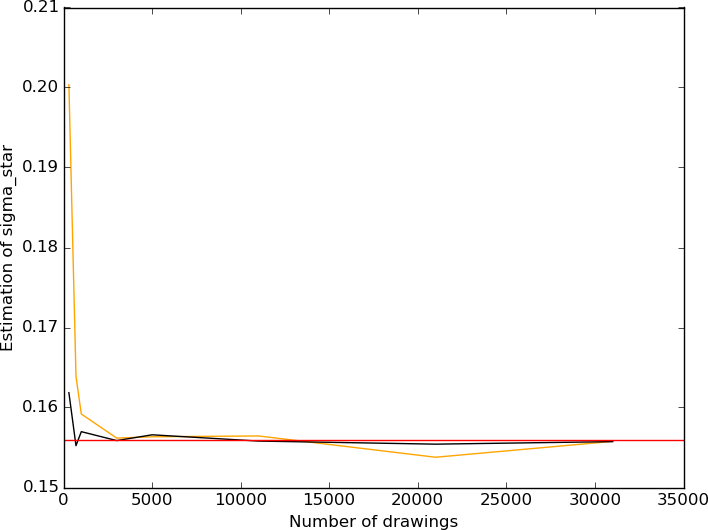
\includegraphics[scale=0.47]{\directory/stratification_reproduce_variance_a.png}
			\subcaption{Méthode a)}
	\end{subfigure}
	\hfill
	\begin{subfigure}[scale=1]{0.45\textwidth}
		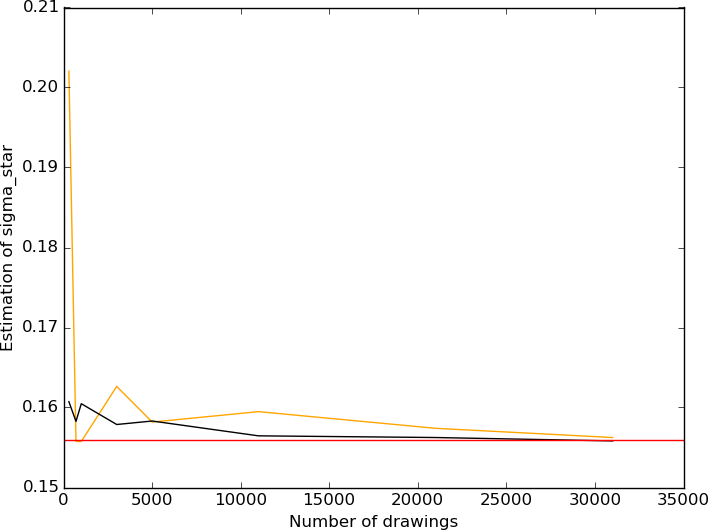
\includegraphics[scale=0.47]{\directory/stratification_reproduce_variance_b.png}
		\subcaption{Méthode b)}
	\end{subfigure}

	
\caption{\small Comparaison entre l'intervalle de confiance estimé à partir de l'estimation de la variance asymptotique $\sigma^{*}$ (en orange) et celui obtenu par simulation Monte Carlo avec 10000 tirages (en noir) pour l'estimation de l'espérance d'une loi normale standard. Les courbes tracées sont estimations de $\sigma^{*}$ (proportionnel à la largeur de intervalle de confiance et la vraie valeur (en rouge)). Avec notre implémentation, la méthode b) semble la moins fiable.}
\label{fig:strat_comparaison_sigma}
\end{figure}

\subsection{Comparaison de la stratification proportionnelle et de la méthode adaptative}

\begin{table}[H]
\centering
	\begin{tabular*}{\textwidth}{@{\extracolsep{\fill}}ccc}
		\hline
		 			    & Stratification proportionnelle 		& Stratification adaptative \\ 
		 			    																	\\
		\hline
		Variance	    & 1.26e-06		                        & 7.82e-07	                \\
		Temps (s)      	& 0.0249		                        & 0.0256                    \\
		Variance*temps	& 3.14e-08                              & 2.00e-08		            \\
		\hline
	\end{tabular*}
\caption{Comparaison des résultats entre les méthodes d'allocation proportionnelles et adaptative pour l'estimation de l'espérance d'une loi normale standard. Nous utilisons 31300 tirages pour la stratification, répartie successivement en 300, 1300, 11300 puis 31300 tirages pour la méthode adaptative. L'expérience est répétée 10000 fois et les valeurs présentés sont les moyennes des résultats obtenus.}
\label{tab:strat_comparaison_proportionnelle_adaptative}
\end{table}

\subsection{Comparaison avec les résultats de \cite{EJ08} pour les options asiatiques}

\begin{table}[H]
\centering
	\begin{tabular*}{\textwidth}{@{\extracolsep{\fill}}ccccccc}
		\hline
			                &   &   & \multicolumn{2}{|c|}{Variance} &                      \\ 
		\hline
		
		d	                & K  & Price  & Adap.    & Prop.    & Ratio Prop. / Adap        \\
		\hline
		\multirow{3}{*}{16} & 45 & 6.05   & 2.63e-08 & 1.08e-07 & 4.11	                    \\
							& 50 & 1.91   & 1.20e-07 & 7.76e-06 & 64.69	                    \\
							& 55 & 0.20   & 5.29e-09 & 4.33e-07 & 81.74	                    \\
	 \hline
		\multirow{3}{*}{64} & 45 & 6.00   & 3.53e-09 & 2.32e-08 & 6.58	                    \\
							& 50 & 1.84   & 1.00e-09 & 3.05e-09 & 3.04                      \\
							& 55 & 0.17   & 6.55e-09 & 7.36e-07 & 112.35	                \\
		\hline
	\end{tabular*}
\caption{Comparaison des allocations proportionnelles et adaptative pour l'exemple du call asiatique. Les ratios trouvés sont environ 2 fois supérieures à ceux de \cite{EJ08}.}
\label{tab:strat_asian_call}
\end{table}

\begin{table}[H]
\centering
	\begin{tabular*}{\textwidth}{@{\extracolsep{\fill}}ccccccc}
		\hline
			                &   &   & \multicolumn{2}{|c|}{Variance} &                      \\ 
		\hline
		
		d	                & K  & Price  & Adap.    & Prop.    & Ratio Prop. / Adap        \\
		\hline
		\multirow{3}{*}{16} & 45 &    &  &  & 	                    \\
							& 50 &    &  &  & 	                    \\
							& 55 &    &  &  & 	                    \\
		\hline
		\multirow{3}{*}{64} & 45 &    &  &  & 	                    \\
							& 50 &    &  &  &                       \\
							& 55 &    &  &  & 	                \\
		\hline
	\end{tabular*}
\caption{Comparaison des allocations proportionnelles et adaptative pour l'exemple du put asiatique avec $S0 = 50$, $r = 0.05$, $\sigma = 0.1$, $T = 1.$ et 100 strates. 1000000 de tirages sont utilisés, répartie progressivement en 100000, 400000, 500000 et 1000000 pour la méthode adaptative.}
\label{tab:strat_asian_put}
\end{table}


\chapter{Comparaison des deux méthodes de réduction de variance sur les exemples de \cite{EJ08}}

\subsection{Loi normale standard}

\subsection{Options asiatiques}

%\begin{figure}[h!]
%	\label{fig:conditionStabilite}
%	\centering
%	\includegraphics[scale=0.75]{}
%	\includegraphics[scale=0.75]{}
%	\caption{}
%\end{figure}

\chapter{Présentation du code C++}


\bibliography{bibliographie}{}
\bibliographystyle{alpha}
\end{document}